\chapter{Southwestern Atlantic Cyclones Energetics Climatology} \label{ch:energetics}

This chapter delves into the energetics of cyclones in the Southwestern Atlantic. The Lorenz Energy Cycle (LEC) was computed for all 7,531 systems with genesis in the ARG, LA-PLATA, and SE-BR regions, as described in Chapter \ref{cyclone_life_cycle}. This extensive dataset, the first of its kind for the South Atlantic region, provides a comprehensive view of the energetics of cyclonic systems near South America. Section \ref{sec:climatology} explores the climatology of these systems over their complete life cycle, while Section \ref{sec:climatology_phases} examines the energetics across each development phase, offering a unique perspective on the energy cycle of cyclonic systems in the region.

\section{Complete Life Cycle Climatology}\label{sec:climatology}

\subsection{Descriptive Statistics} \label{sec:statistics_complete}

This section provides exploratory statistics for each term of the LEC, covering the systems' complete life cycle. The aim is to offer a comprehensive view of the systems' energetics while identifying the main differences among the terms. Table \ref{tab:lec_stats} contains exploratory statistical metrics for these terms. Figure \ref{fig:boxplot_energy_total} presents the boxplots for all LEC components, where each panel depicts a distinct group of terms: (A) energy, (B) conversion, (C) boundary, (D) generation/dissipation terms, and (E) budgets. Figures \ref{fig:ridge_plot_Energy_Terms_total}, \ref{fig:ridge_plot_Conversion_Terms_total}, \ref{fig:ridge_plot_Boundary_Terms_total}, \ref{fig:ridge_plot_Generation_Dissipation_Terms_total}, and \ref{fig:ridge_plot_Budgets_total} display these groups of terms' density distributions, respectively.

\begin{figure}[!htbp]
\centering
\includegraphics[width=\textwidth]{figs_5/box_plot_Total_all_groups.png}
\caption[Box plots - Complete Lifecycle]{Box plots of each group of energetic terms, for the systems complete lifecycle. Each subplot represents a different group of terms: (A) Energy Terms, (B) Conversion Terms, (C) Boundary Terms, (D) Generation/Dissipation Terms, (E) Budgets. The box plots display the distribution of values for each term within the specified group, with the horizontal line indicating the median, the box representing the interquartile range (IQR), and the whiskers extending to 1.5 times the IQR. Outliers are shown as individual points.}
\label{fig:boxplot_energy_total}
\end{figure}

For the energy terms, the values for $K_Z$ are an order of magnitude higher than the others for all metrics analyzed (Table \ref{tab:lec_stats}). Despite the high standard deviation (std) and quantile (Q) values indicating substantial variability, this can be attributed to the presence of numerous outliers (Figure \ref{fig:boxplot_energy_total}a). Most values for $K_Z$ peak between 15 and 17 $\times 10^5 \, J \, m^{-2}$ (Figure \ref{fig:ridge_plot_Energy_Terms_total}c). In contrast, $A_Z$ presents relatively moderate mean and median values, with a right-skewed distribution and significant spread (Figure \ref{fig:ridge_plot_Energy_Terms_total}a). The notable outliers (Figure \ref{fig:boxplot_energy_total}a) suggest periods of unusually high energy values.

Overall, the eddy energy terms ($A_E$ and $K_E$) exhibit less variability and fewer outliers compared to the zonal energy terms ($A_Z$ and $K_Z$) (Figure \ref{fig:boxplot_energy_total}a). They also have smaller mean and median values (Table \ref{tab:lec_stats}). Although both eddy energy terms peak close to each other, the distribution of $A_E$ is more concentrated around the median (Figure \ref{fig:ridge_plot_Energy_Terms_total}b), with a narrower interquartile range (IQR) and lower standard deviation, suggesting it is more stable and consistent over time. In contrast, $K_E$ presents a more right-skewed distribution than $A_E$ (Figure \ref{fig:ridge_plot_Energy_Terms_total}d).


\begin{figure}[!htbp]
\centering
\includegraphics[width=\textwidth]{figs_5/ridge_plot_Energy_Terms_total.png}
\caption[Density Plots - Energy Terms]{Density plots for energy terms $A_Z$ (A), $A_E$ (B), $K_Z$ (C), and $K_E$ (D). The units are $J m^{-2}$.}
\label{fig:ridge_plot_Energy_Terms_total}
\end{figure}

While the mean values of $A_E$ and $K_E$ are generally in agreement with previous studies, the values of $K_Z$ and $A_Z$ differ significantly \citep[e.g.,]{michaelides1999quasi,veiga2008analysis,dias2011energy,pezza2014large}. \citet{li2007lorenz} and \citet{veiga2013global}, analyzing global LEC values, found mean $K_Z$ values for the Southern Hemisphere of approximately $10$ and $15.8 \times 10^5 \, J \, m^{-2}$ and mean $A_Z$ values of approximately $40$ and $16 \times 10^5 \, J \, m^{-2}$, respectively. Analyzing the LEC of extratropical cyclones primarily in the Northern Hemisphere, \citet{smith1980energetics} found mean $K_Z$ and $A_Z$ values of $15$ and $25 \times 10^5 \, J \, m^{-2}$, respectively. Meanwhile, \citet{black2013universal}, for explosive cyclogenesis in the Northwest Pacific region, found mean $A_Z$ and $K_Z$ values of approximately $30$ and $48 \times 10^5 \, J \, m^{-2}$, respectively. Here, $K_Z$ and $A_Z$ presented mean values of $28.55$ and $5.55 \times 10^5 \, J \, m^{-2}$, respectively.


\begin{table}[!htbp]
\centering
\caption[Summary Statistics of Lorenz Energetics Components]{Summary Statistics of Lorenz Energetics Components: mean, median, standard deviation (std), 20th percentile (Q20), 80th percentile (Q80), interquantile range (IQR), and range. The IQR measures the range within which the central 50\% of the values fall, while the range is computed as the difference between the maximum and minimum values. The units for the energy terms ($A_Z$, $A_E$, $K_Z$, and $K_E$) are $10^5 \, J \, m^{-2}$ and $W \, m^{-2}$ for the remaining terms.}
\label{tab:lec_stats}
\begin{tabular}{lrrrrrrr}
\toprule
Term & Mean & Median & Std & Q20 & Q80 & IQR & Range \\
\midrule
Az & 5.55 & 4.68 & 3.71 & 2.41 & 8.30 & 5.89 & 36.46 \\
Ae & 1.62 & 1.24 & 1.20 & 0.69 & 2.37 & 1.68 & 11.07 \\
Kz & 28.55 & 26.19 & 15.10 & 15.52 & 40.16 & 24.64 & 114.55 \\
Ke & 3.70 & 2.95 & 2.62 & 1.73 & 5.22 & 3.49 & 24.81 \\
Cz & 0.52 & 0.38 & 4.85 & -2.69 & 3.72 & 6.41 & 86.70 \\
Ca & 0.93 & 0.46 & 1.57 & -0.06 & 1.79 & 1.84 & 19.78 \\
Ck & -3.56 & -1.63 & 9.51 & -7.41 & 1.11 & 8.52 & 206.43 \\
Ce & 3.84 & 2.47 & 4.92 & 0.33 & 6.97 & 6.64 & 54.74 \\
BAz & 3.54 & 2.03 & 7.67 & -1.35 & 8.23 & 9.57 & 175.05 \\
BAe & 0.58 & 0.16 & 4.40 & -1.62 & 2.75 & 4.37 & 75.72 \\
BKz & -7.93 & -5.53 & 31.75 & -29.51 & 12.06 & 41.57 & 445.63 \\
BKe & 0.47 & 0.08 & 8.59 & -3.67 & 4.40 & 8.07 & 146.87 \\
$B\Phi Z$ & 63.87 & 49.25 & 128.05 & -24.60 & 156.65 & 181.25 & 1419.08 \\
$B\Phi E$ & 39.66 & 31.19 & 126.50 & -46.44 & 132.10 & 178.54 & 1353.99 \\
Gz & -0.31 & -0.17 & 2.66 & -1.82 & 1.14 & 2.96 & 68.74 \\
Ge & 1.17 & 0.56 & 3.14 & -0.47 & 2.79 & 3.26 & 58.39 \\
$\frac{\partial A_Z}{\partial t}$ & -0.07 & -0.14 & 4.46 & -2.66 & 2.31 & 4.97 & 106.39 \\
$\frac{\partial A_E}{\partial t}$ & -0.23 & -0.10 & 1.92 & -1.14 & 0.74 & 1.88 & 48.19 \\
$\frac{\partial K_Z}{\partial t}$ & 1.59 & 0.75 & 13.38 & -7.13 & 10.40 & 17.53 & 251.24 \\
$\frac{\partial K_E}{\partial t}$ & 0.28 & 0.12 & 3.18 & -1.53 & 2.09 & 3.62 & 61.50 \\
RGz & -2.17 & -1.00 & 7.60 & -6.69 & 2.31 & 9.01 & 220.06 \\
RKz & 12.56 & 8.69 & 40.49 & -13.89 & 40.08 & 53.96 & 561.24 \\
RGe & 2.10 & 1.20 & 5.15 & -0.84 & 5.28 & 6.12 & 97.25 \\
RKe & -7.59 & -4.63 & 10.62 & -13.68 & -0.45 & 13.23 & 138.42 \\
\bottomrule
\bottomrule
\end{tabular}
\end{table}

The scarcity of results for a comprehensive set of systems hinders drawing decisive conclusions about the behavior of the $A_Z$ and $A_E$ terms in cyclonic occurrences, while individual cases offer high variability, as indicated by case studies \citep[e.g.,]{brennan1980zonal,dias2011energy,pezza2014large} and the higher variability in the data (Table \ref{tab:lec_stats}). However, several observations can be made:  1) When compared to global energetics, cyclonic systems present higher $K_Z$ values. This is expected because $K_Z$ involves a zonal average of the wind components (Equation \ref{eq:KZ}), and global averages would yield smaller values than those for limited areas closer to the cyclonic center, often associated with high-level jets; 2) Limited areas provide smaller $A_Z$ values than hemispheric averages, due to the reduced meridional temperature and static stability gradients (Equation \ref{eq:AZ}). These effects are even more evident in the current study, as the computational domain following the system focuses on the environmental dynamics surrounding it, thus capturing overall higher wind speeds through the atmosphere and smaller meridional temperature gradients. A similar effect is noted in \citet{michaelides1999quasi}; 3) Furthermore, the literature shows that the magnitude and sign of the conversion, boundary, generation, and dissipation terms exhibit high variability across different systems and development phases \citep[e.g.,]{brennan1980zonal,smith1980energetics,michaelides1987limited,bulic2006limited,dias2011energy,black2013universal}, complicating comparisons of the overall values presented here with individual cases.

For the conversion terms, while $C_Z$, $C_A$, and $C_E$ are positive on average and in median values, $C_K$ is negative (Table \ref{tab:lec_stats}). For $C_A$ and $C_E$, there is a relatively narrow spread around the median, with some significant outliers (Figure \ref{fig:boxplot_energy_total}b). $C_A$, showing a distribution centered around zero with both negative and positive values (Figure \ref{fig:ridge_plot_Conversion_Terms_total}b), indicates alternating periods of energy transfer in both directions, predominantly from $A_Z$ to $A_E$. Meanwhile, $C_E$ has a left-skewed distribution (Figure \ref{fig:ridge_plot_Conversion_Terms_total}d) and higher Q20 and IQR values, suggesting a more consistent positive net conversion. 

The $C_K$ term exhibits a wide distribution peaking at negative values (Figure \ref{fig:ridge_plot_Conversion_Terms_total}c), with a significant negative mean and median, indicating a dominant net conversion from $K_Z$ to $K_E$. The large range and standard deviation, along with the presence of significant outliers, suggest substantial variability in this conversion process. Lastly, $C_Z$ presents the most distinctive behavior, with values centered around zero but peaking at both positive and negative values (Figure \ref{fig:ridge_plot_Conversion_Terms_total}a). However, the higher peak at positive values along with the positive mean and median values indicate a preference for conversion from $A_Z$ to $K_Z$. 

The overall values presented here indicate that, throughout the systems' complete lifecycle, $K_E$ tends to receive energy from $A_E$ and, in most cases, from $K_Z$ as well, although there are instances where $C_K$ tends to be positive. There is also a general tendency for $A_Z$ to be converted to $A_E$, albeit with a lower magnitude. Meanwhile, although $C_Z$ can be positive, negative, or neutral, the predominant tendency is for conversion from $A_Z$ to $K_Z$.

\begin{figure}[!htbp]
\centering
\includegraphics[width=\textwidth]{figs_5/ridge_plot_Conversion_Terms_total.png}
\caption[Density Plots - Conversion Terms]{Density plots for conversion terms $C_Z$ (A), $C_A$ (B), $C_K$ (C), and $C_E$ (D). The units are $W m^{-2}$.}
\label{fig:ridge_plot_Conversion_Terms_total}
\end{figure}

There is a notable difference between the boundary flux terms ($BA_Z$, $BA_E$, $BK_Z$, $BK_E$) and the boundary pressure work terms ($B\Phi Z$ and $B\Phi E$) (Table \ref{tab:lec_stats}). For the boundary flux terms, $BA_Z$ presents the highest mean and median values, while $BK_Z$ has the lowest. $BA_E$ and $BK_E$ have mean and median values closer to zero. The $BA_Z$ term exhibits moderate variability, with a wide distribution around the median (Figure \ref{fig:ridge_plot_Boundary_Terms_total}a) and few outliers (Figure \ref{fig:boxplot_energy_total}c), a similar pattern to $BK_E$ (Figure \ref{fig:ridge_plot_Boundary_Terms_total}d). $BA_E$, in turn, displays the lowest variability among the boundary terms, with most values peaking near zero (Figure \ref{fig:ridge_plot_Boundary_Terms_total}b). Meanwhile, $BK_Z$ presents the most distinctive behavior, exhibiting high variability, with a wide distribution (Figure \ref{fig:ridge_plot_Boundary_Terms_total}c) and numerous outliers. Its values range from the most negative to the most positive among the boundary terms, indicating an overall tendency for the exportation of zonal kinetic energy, supported by its negative mean and median values.

On the other hand, the boundary pressure work terms present similar behavior, with very high mean and median values, especially $B\Phi Z$, and displaying two peaks: one on negative values (with a higher peak for the $B\Phi E$ term) and another, which displays higher densities, on positive values (Figure \ref{fig:ridge_plot_Boundary_Terms_total}e and \ref{fig:ridge_plot_Boundary_Terms_total}f). Both terms present low Q20 and high Q80 values, indicating that although they generally contribute to the appearance of energy in the $K_Z$ and $K_E$ terms, there are instances where they contribute negatively. For all metrics presented, they exhibit the highest values in magnitude across all terms. As \citet{brennan1980zonal} argued, these high values are associated with minor errors in the geopotential height field that can escalate. Although ERA5 presents the most modern reanalysis product offering homogeneous high-resolution data, systematic errors might be present, especially in regions with low data coverage, such as over the oceans and high altitudes \citep{hersbach2020era5}. As most studies do not compute these terms as residuals and thus do not present the values (for instance, none of the studies presented in Section \ref{sec:lec_cyclones} do so), direct comparison of the values obtained here with the literature is hindered.

\begin{figure}[!htbp]
\centering
\includegraphics[width=\textwidth]{figs_5/ridge_plot_Boundary_Terms_total.png}
\caption[Density Plots - Boundary Terms]{Density plots for boundary terms $BA_Z$ (A), $BA_E$ (B), $BK_Z$ (C), $BK_E$ (D), $B\Phi Z$ (E), and  $B\Phi E$ (F). The units are $W m^{-2}$.}
\label{fig:ridge_plot_Boundary_Terms_total}
\end{figure}

%% !
Although the energy budgets are computed using residuals (which include the boundary pressure work terms), the generation terms are also analyzed as they serve both as an overall evaluation of the generation residual terms and because, in future sections, they will be used for understanding the systems' dynamics. Both $G_Z$ and $G_E$ present a similar distribution, displaying low variability (Figure \ref{fig:ridge_plot_Boundary_Terms_total}), with most values peaking near zero and with minor peaks on both positive and negative values (Figures \ref{fig:ridge_plot_Generation_Dissipation_Terms_total}a and \ref{fig:ridge_plot_Generation_Dissipation_Terms_total}b). However, $G_E$ presents a higher density of positive values, which is reflected in its higher mean and median values than $G_Z$ and higher Q80 values (Table \ref{tab:lec_stats}). 

For the generation residual terms, both present three peaks - at positive, neutral, and negative values - but while $RG_Z$ has the highest density around negative values, $RG_E$ peaks at positive values (Figures \ref{fig:ridge_plot_Generation_Dissipation_Terms_total}c and \ref{fig:ridge_plot_Generation_Dissipation_Terms_total}e). This results in $RG_E$ presenting positive mean and median values, despite a minor peak at negative values - which reflects in a negative Q20 value - indicating that its contribution to $\frac{\partial A_E}{\partial t}$ is mainly positive, with situations where this term contributes negatively. For $RG_Z$, the opposite is noted, with negative mean and median values, but a minor peak at positive values - reflected in a positive Q80 - indicating it mainly contributes negatively to $\frac{\partial A_Z}{\partial t}$, with situations where this term contributes positively.

Furthermore, while $RK_Z$ presents higher positive mean and median values, it also shows high variability and numerous outliers (Figure \ref{fig:boxplot_energy_total}d). It presents a distinctive density distribution, with two marked peaks, one for positive and the other for negative values (Figure \ref{fig:ridge_plot_Generation_Dissipation_Terms_total}d). This is reflected in its negative Q20 and positive Q80 values, with a high IQR. Therefore, although it mostly contributes positively to $\frac{\partial K_Z}{\partial t}$, there are also significant instances where it contributes negatively. $RK_E$, on the other hand, presents mean and median values peaking at negative values (Figure \ref{fig:ridge_plot_Generation_Dissipation_Terms_total}f). Therefore, it mostly contributes negatively to $\frac{\partial K_E}{\partial t}$, acting as a sink for $K_E$.

\begin{figure}[!htbp]
\centering
\includegraphics[width=\textwidth]{figs_5/ridge_plot_Generation_Dissipation_Terms_total.png}
\caption[Density Plots - Generation Terms]{Density plots for generation terms $G_Z$ (A) and $G_E$ (B); and residual terms $RG_Z$ (C), $RK_Z$ (D), $RG_E$ (E), and $RK_E$ (F). The units are $W m^{-2}$.}
\label{fig:ridge_plot_Generation_Dissipation_Terms_total}
\end{figure}

Among the budget terms, APE terms ($\frac{\partial A_Z}{\partial t}$ and $\frac{\partial A_E}{\partial t}$) present negative mean and median values, while the kinetic energy terms ($\frac{\partial K_Z}{\partial t}$ and $\frac{\partial K_E}{\partial t}$) are positive, although all of them exhibit negative Q20 values and positive Q80 values, indicating variability among the analyzed systems (Table \ref{tab:lec_stats}).  $\frac{\partial A_E}{\partial t}$ has the lowest variability, with the smallest IQR and range values, fewest outliers (Figure \ref{fig:boxplot_energy_total}), and the highest peak density centered around zero (Figure \ref{fig:ridge_plot_Budgets_total}b). This indicates that while in most cases there is an overall tendency for $A_E$ to be neutral, there are also occurrences of positive and negative increments.

In contrast, $\frac{\partial A_Z}{\partial t}$ and $\frac{\partial K_E}{\partial t}$ display similar density distributions (Figure \ref{fig:ridge_plot_Budgets_total}a and \ref{fig:ridge_plot_Budgets_total}d), with peaks at negative, neutral, and positive values. $\frac{\partial A_Z}{\partial t}$ has a higher peak at negative values, indicating a tendency for $A_Z$ to decrease, while $\frac{\partial K_E}{\partial t}$ peaks at positive values, reflecting a tendency for $K_E$ to increase. However, both terms also show instances of neutrality and opposite trends. Lastly, $\frac{\partial K_Z}{\partial t}$ exhibits a unique behavior with two prominent peaks at opposite extremes (Figure \ref{fig:ridge_plot_Budgets_total}c). This term has the lowest Q20 and the highest Q80, IQR, and range values, indicating that $K_Z$ tends to exhibit extreme changes — either significant increases or decreases — with a smaller tendency to remain neutral.


\begin{figure}[!htbp]
\centering
\includegraphics[width=\textwidth]{figs_5/ridge_plot_Budgets_total.png}
\caption[Density Plots - Budget Terms]{Density plots for budget terms $\frac{\partial A_Z}{\partial t}$ (A) and $\frac{\partial A_E}{\partial t}$ (B); $\frac{\partial K_Z}{\partial t}$ (C), and $\frac{\partial K_E}{\partial t}$ (D). The units are $W m^{-2}$.}
\label{fig:ridge_plot_Budgets_total}
\end{figure}

\subsection{Mean Energy Cycle}\label{sec:lec_mean}

Figure \ref{fig:lec_mean_values} illustrates the LEC for the mean values of each term. Although, due to the high variability presented for the distinct terms, as shown previously, such result should be looked upon with care, it can provide an overview of the mean energy fluxes on the analyzed systems. Additionally, $G_Z$ and $G_E$ terms are used for a more physically based interpretation, although the budgets were computed using their respective residuals. Since the residual terms integrated these components, the presented budgets may not perfectly balance positive and negative energy fluxes due to the finite differences method used, which also incorporates numerical errors.

\begin{figure}[!htbp]
\centering
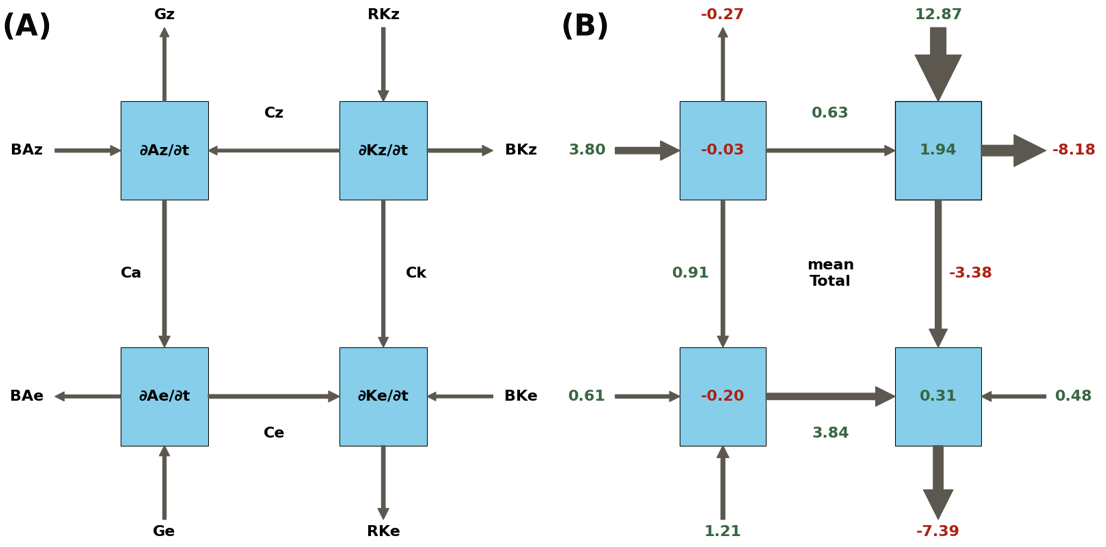
\includegraphics[width=\textwidth]{figs_5/lec_mean_values.pdf}
\caption[LEC - Mean Life Cycle]{Representation of the LEC, with arrows denoting positive energy conversions (A) and mean values of the Lorenz Energy Cycle (LEC) terms (B). Each blue box represents an energy component, with arrows showing the direction of energy flow. The numbers adjacent to the arrows indicate the magnitude and direction of the energy flux, with green indicating positive values and red indicating negative values.}
\label{fig:lec_mean_values}
\end{figure}

The mean values indicate an overall tendency for both APE terms to decrease over time. The decreases in $A_Z$ are primarily due to conversions to $A_E$ ($C_A > 0$, Figure \ref{fig:Ca}), which is an expected result. As discussed in Section \ref{track_method}, most cyclones in the dataset are extratropical, which have the final cause of diminishing Equator-Pole temperature gradients (Section \ref{final_causes}), i.e., reducing $A_Z$. Additionally, there are overall losses of $A_Z$ due to the $G_Z$ term, indicating either anomalous heating in cool regions or anomalous cooling in warm regions caused by the eddy's meridional heat transport. Imports of $A_Z$ are also observed through the $BA_Z$ term. For the $A_E$ term, there are decreases over time. Despite influxes from $C_A$, diabatic processes ($G_E > 0$) and imports of energy ($BA_E > 0$), most of its energy is converted to $K_E$ ($C_E > 0$) due to enhanced zonal temperature gradients.

The mean values indicate both forms of kinetic energy increasing over time. The increase in $K_Z$ - which is the greatest among the budget terms - primarily stems from influxes from the residual term ($RK_Z > 0$). Although the inclusion of numerical errors hinders the interpretation of the residual term, Section \ref{sec:climatology} indicates that $B\Phi_Z$ often presents large values, suggesting that this energy influx might be related to the generation of kinetic energy - by the zonal jets - towards the cyclone's central low pressure. Meanwhile, a great part of $K_Z$ energy is exported outside the domain ($BK_Z < 0$), while a minor part is converted to $K_E$ through the barotropic conversion term ($C_K < 0$). Only negligible amounts are converted from $A_Z$. Finally, $K_E$ displays increases over time, driven mostly by conversion from $A_E$, but also with significant contributions from $C_K$. Notably, $RK_E$ presents high magnitudes, possibly indicating the dissipation of this energy. The importation of $K_E$ is almost negligible.

In summary, for the mechanisms related to eddy growth, it can be seen that the mean environment energetics related to the cyclones in the SESA region indicate that both the baroclinic and barotropic chains are active. This indicates that the eddies gain energy from both meridional temperature gradients as well as from horizontal wind shear. Moreover, diabatic processes contribute to increasing the eddy APE, thus supporting the moist baroclinic chain. Finally, the main sink for eddy energy is the residual term, possibly associated with dissipation by frictional forces.

\subsection{EOFs}\label{sec:eof_complete}

The results presented in Section \ref{sec:statistics_complete} demonstrate that the LEC terms exhibit high variability. Even a view of the LEC for the mean values can be problematic, as each term spans a wide range of possible values, often with varying signs. Therefore, delineating an overall picture of the LEC for the analyzed systems is not a trivial task. To help address this issue, an empirical orthogonal function (EOF) analysis is used. It is important to note that the values represent anomalies rather than the actual magnitudes of the energy cycle components.

Figure \ref{fig:variance_explained} illustrates the proportion of variance in the dataset that is explained by each of the first eight Empirical Orthogonal Functions (EOFs). The first EOF accounts for the largest share of the variance, explaining 28.3\%, indicating it captures the most significant pattern in the data. The second and third EOFs both explain around 11\% of the variance, showing that they also represent notable patterns but with less influence compared to the first EOF. The subsequent EOFs explain progressively smaller proportions of the variance: 8.2\% for the fourth, 7.4\% for the fifth, 5.9\% for the sixth, 5.2\% for the seventh, and 4.4\% for the eighth. Together, these eight EOFs capture the primary modes of variability within the dataset. Usually, the principal components (PCs, not shown) represent the temporal evolution of the signal magnitude of each EOF. However, in this context, they would merely represent the signal magnitude across the distinct cyclones and therefore do not represent any physical feature.

\begin{figure}[!htbp]
\centering
\includegraphics[width=0.9\columnwidth,angle=0]{figs_5/variance_explained.png}
\caption[EOF - Explained Variance]{Proportion of variance in the dataset explained by the first eight Empirical Orthogonal Functions (EOFs).}
\label{fig:variance_explained}
\end{figure}

For the EOF1 (Figure \ref{fig:eofs_total}), most terms are in general agreement with the signal for mean values presented in Figure \ref{fig:lec_mean_values}, indicating an enhancement of the average behavior. The exceptions to this are the $C_Z$, $BA_E$ and $A_E$ budget terms; however, the anomaly signal magnitude is lower than what is found in the mean values, indicating that for the first variability mode, there is no reversal in the sign of the observed values. In general, this result confirms the observation that the overall behavior of the environmental energetics related to the cyclones in the SESA region is associated with the moist baroclinic chain, acting together with barotropic conversions.

For the EOF2, although many terms present anomalies with a reversed sign compared to the mean values, the magnitude of most of them is not high enough to signal a reversal in the energy flux direction or represent significant changes in the overall behavior. However, some significant changes can be noted in certain terms. For instance, the terms $\frac{\partial A_Z}{\partial t}$ and $\frac{\partial K_E}{\partial t}$ present an enhancement of the mean behavior. For $\frac{\partial A_Z}{\partial t}$, this is mostly linked to the further diminishing of $G_Z$ in the EOF2, while for $\frac{\partial K_E}{\partial t}$, this is primarily associated with enhanced imports from $BK_E$, with minor contributions from the enhanced moist baroclinic chain. Although the signal is weak, EOF2 also presents a small weakening of the barotropic conversions.

\begin{figure}[!htbp]
\centering
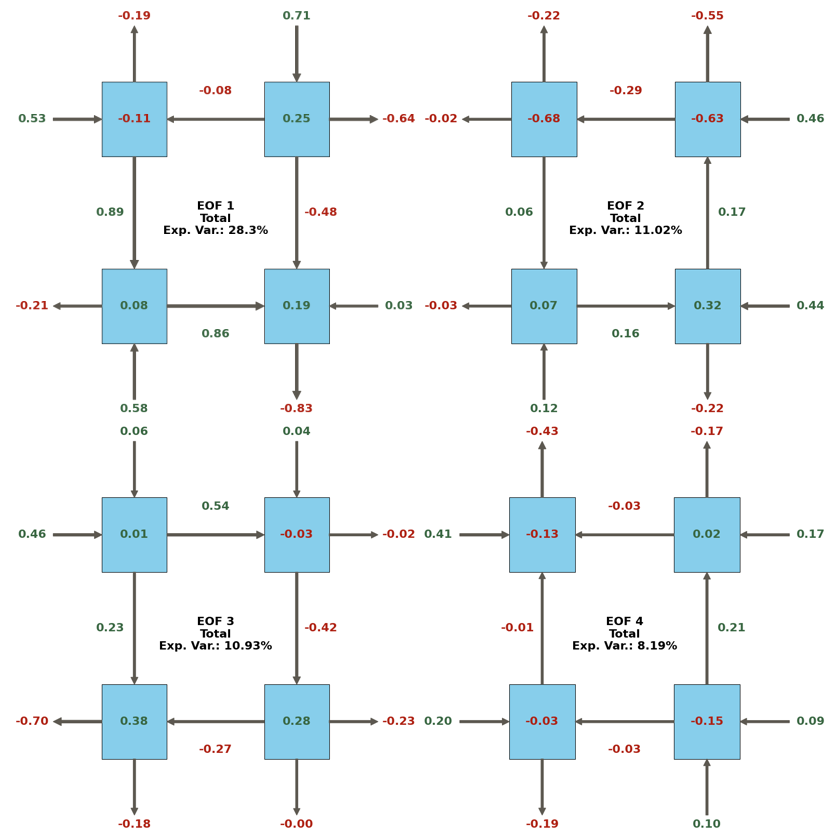
\includegraphics[width=\textwidth]{figs_5/eofs_total.pdf}
\caption[EOF Analysis - Total Lifecycle]{EOF Analysis of Lorenz Energy Cycle (LEC) Terms, illustrating the anomalies in energy fluxes: EOF1 (A), EOF2 (B), EOF3 (C) and EOF4 (D). 
The numbers adjacent to the arrows denote the magnitude and direction of the anomaly, with green indicating positive values and red indicating negative values.}
\label{fig:eofs_total}
\end{figure}

For the EOF3, it is evident that the signal for $\frac{\partial A_E}{\partial t}$ has a higher magnitude and opposite sign compared to the mean value. The positive budget for $A_E$ is mostly associated with enhanced conversion from $A_Z$ and a reduction in the conversions to $K_E$, although there are strong reductions in the $BA_E$, which indicate a reversal in this term's sign. For $\frac{\partial K_E}{\partial t}$, there is also a significant signal for the enhancement of the positive budget, primarily associated with the enhancement of the barotropic conversion by the $C_K$ term. 

In general, while the EOF2 presents an enhancement of the moist baroclinic chain, with a diminishment of barotropic conversions, the EOF3 presents the opposite behavior. The EOF4, in turn, presents a reversal in sign for most terms compared to the mean values. However, for most of them, the signal is not high enough to represent a significant reversal of the mean values. The most notable distinction is in the $G_Z$ term, which becomes even more negative. 

The following EOFs continue to exhibit such small signals, presenting only minor deviations from the mean behavior of the LEC. Therefore, they will not be further discussed. The EOF analysis presented here demonstrates that, although there is high variability in the dataset, with individual cases presenting overall energetics deviating from the mean values, the mean energetics or the mean state of the cyclones is much stronger than the fluctuations or variations captured by the EOFs (Appendix \ref{ap03} contains the reconstructed EOFs). This might be intrinsically linked to the EOFs being calculated for the entire life cycle of the systems, with distinct dynamical processes acting at different development stages. Next sections will explore to what extent the results presented can be applied to each development phase or if the distinct phases will reveal further details about the energetics of the cyclones in SESA region.

\section{Climatology Across Life Phases}\label{sec:climatology_phases}

\subsection{Descriptive Statistics}\label{sec:statistics_phases}

Although Sections \ref{sec:statistics_complete} and \ref{sec:eof_complete} provide an overview of the systems' energetics, their results apply to the complete life cycle. As distinct dynamical processes might act at different development stages, it is expected that different phases of the cyclone's life cycle will present different overall energy cycles. Here, the cyclones' lifecycle was dissected using the Cyclophaser program to investigate the LEC for each phase individually, aiming to understand which processes dominate in each of them.

The first step was to assess whether the different development phases exhibit statistically significant differences among themselves. Table \ref{tab:lec_stats_phases} presents the p-values for the normality, homogeneity, and significance tests employed. Normality was assessed using the Shapiro-Wilk test, and homogeneity was assessed using Levene's test. For all terms, the p-values were well below the 0.05 threshold, indicating that the data significantly deviate from normality and that their variances differ significantly across the phases. Therefore, to determine statistically significant differences between the phases, we employed the non-parametric Kruskal-Wallis (KW) test. The results indicated that the differences in the LEC terms among the phases are statistically significant.  While post-hoc Dunn's tests could be conducted to identify which specific phases differ if the Kruskal-Wallis test is significant, this would involve a combinatorial analysis of pairs among seven phases for all 17 terms in the LEC. Such an analysis would be impractical. Consequently, the statistically significant results from the KW test were deemed sufficient for proceeding with the analysis.

\begin{table}[!htbp]
\centering
\caption[Statistical Analysis Results for Different Phases]{Statistical Analysis Results for Different Phases. The table shows the p-values for the Kruskal-Wallis (KW) test, the Shapiro-Wilk normality test, and Levene's test for homogeneity of variances. The Kruskal-Wallis test is used here due to non-normality or heterogeneity of variances in the data, indicating significant differences among phases if the p-value is less than 0.05.}
\label{tab:lec_stats_phases}
\begin{tabular}{lrrr}
\toprule
\textbf{Term} & \makecell{\textbf{KW} \\ \textbf{p-value}} & \makecell{\textbf{Normality} \\ \textbf{p-value}} & \makecell{\textbf{Homogeneity} \\ \textbf{p-value}} \\
\midrule
Az & 5.16e-273 & 2.86e-50 & 5.54e-67 \\
Ae & 6.51e-283 & 1.24e-57 & 3.49e-111 \\
Kz & 2.30e-22 & 3.08e-36 & 1.80e-46 \\
Ke & 0.00e+00 & 3.05e-55 & 6.78e-269 \\
Cz & 1.01e-48 & 1.79e-34 & 1.14e-134 \\
Ca & 7.46e-192 & 5.32e-57 & 5.71e-85 \\
Ck & 1.64e-92 & 5.90e-62 & 0.00e+00 \\
Ce & 0.00e+00 & 6.43e-52 & 1.84e-189 \\
BAz & 6.58e-79 & 1.14e-54 & 8.02e-39 \\
BAe & 1.66e-282 & 1.92e-51 & 5.02e-137 \\
BKz & 7.56e-05 & 1.71e-38 & 2.54e-54 \\
BKe & 2.03e-118 & 6.67e-60 & 1.92e-76 \\
$B\Phi Z$ & 2.30e-45 & 4.71e-28 & 5.33e-105 \\
$B\Phi E$ & 6.89e-39 & 2.31e-27 & 3.23e-94 \\
Gz & 1.50e-48 & 9.91e-50 & 0.00e+00 \\
Ge & 0.00e+00 & 2.70e-58 & 6.95e-256 \\
RGz & 7.43e-164 & 5.41e-54 & 1.09e-148 \\
RKz & 5.09e-06 & 1.22e-35 & 2.78e-69 \\
RGe & 1.27e-179 & 4.83e-47 & 1.77e-122 \\
RKe & 1.84e-267 & 9.33e-54 & 7.03e-205 \\
$\frac{\partial A_Z}{\partial t}$ & 2.58e-221 & 2.52e-50 & 0.00e+00 \\
$\frac{\partial A_E}{\partial t}$ & 3.85e-212 & 1.51e-53 & 0.00e+00 \\
$\frac{\partial K_Z}{\partial t}$ & 1.33e-108 & 3.36e-44 & 3.67e-194 \\
$\frac{\partial K_E}{\partial t}$ & 0.00e+00 & 2.65e-55 & 0.00e+00 \\
\bottomrule
\end{tabular}
\end{table}

The next step is to investigate the overall behavior of each term across distinct development phases through their density distributions. Beyond energy terms, the focus will be on the overall energy flux direction, providing a proxy for understanding the dynamical forcing related to the development of cyclonic systems throughout their life cycle. Finally, a summary of the main findings along with interpretations drawn from the results is presented at the end of this section.

Figure \ref{fig:ridge_plot_Energy} displays the density plots for the energy terms for each development phase. It can be observed that the overall shapes of the distributions within the same term are similar, mirroring the distribution for the complete life cycle (Section \ref{sec:statistics_complete}), with minor differences across each specific phase. For $A_Z$ (Figure \ref{fig:ridge_plot_Energy}a), every phase presents maximum densities centered between 2 and 3 $15^5 J m^{-2}$, but displays right-skewed distributions, indicating high variability and the occasional occurrence of extremely high values. Mature phases (1 and 2) exhibit sharper peaks, while intensification (1 and 2) and incipient phases present broader peaks. An overall trend, indicated by both mean and median values, shows $A_Z$ decreasing from the incipient to the mature phase and increasing again through the decay phase. The same trend is observed during secondary development: it decreases from intensification 2 to mature 2 and then increases again at decay 2. Notably, despite this increase during the decay phase, the mean and median values are lower than the initial values, and even lower during the secondary development. This overall trend displayed by $A_Z$ throughout the cyclone's life cycle aligns with the discussion at the end of Section \ref{sec:statistics_complete} and in Section \ref{final_causes}: extratropical cyclones aim to balance global temperature, diminishing temperature gradients (i.e., $A_Z$).

\begin{figure}[!htbp]
\centering
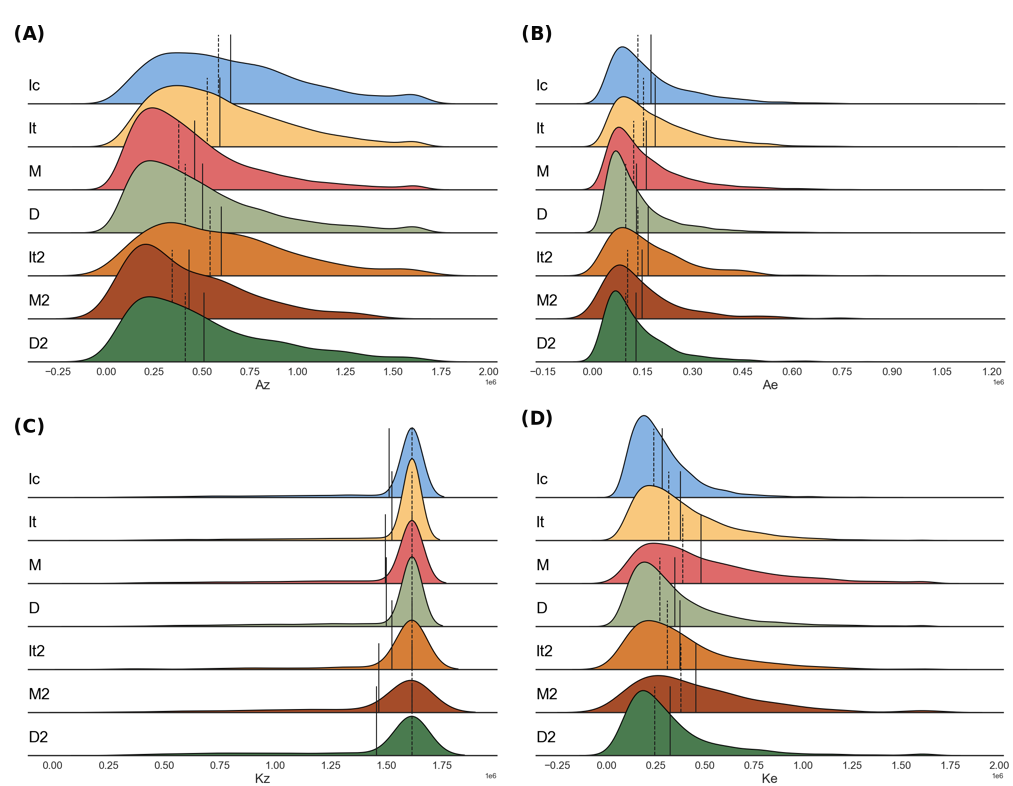
\includegraphics[width=\textwidth]{figs_5/ridge_plot_Energy Terms.pdf}
\caption[Density Plots - Energy Terms]{Density plots for energy terms $A_Z$ (A), $A_E$ (B), $K_Z$ (C), and $K_E$ (D), for each development phase: incipient (Ic), intensification (It), mature (M), decay (D) and the secondary development phases (indicated by "2"). The solid vertical lines indicate the mean values for a given phase while the dashed lines, the median values. The units are $W m^{-2}$.}
\label{fig:ridge_plot_Energy}
\end{figure}

For $A_E$ (Figure \ref{fig:ridge_plot_Energy}b), the densities are less skewed, with sharper peaks compared to $A_Z$, indicating lower variability and fewer extreme values. Most values peak between 0.5 and 1 $15^5 J m^{-2}$, and the mean and median values show an overall increase from the incipient to the intensification phase, where $A_E$ reaches its highest values, followed by a consistent decrease until the decay phase. $A_E$ increases again during the second intensification phase and then decreases from the second mature phase to the decay phases. This pattern suggests that after genesis, the eddies initiate the conversion from meridional to zonal temperature gradients, which peak during intensification and diminish afterward. The lower mean and median values at the decay phases compared to the beginning of each life cycle indicate that the eddies not only diminish the zonal temperature gradients but also reduce them to levels lower than their initial states.

The $K_Z$ term densities present narrow peaks with long tails towards low values, mirroring the distribution for the total phase (Figure \ref{fig:ridge_plot_Energy}c). For all phases, the distributions peak at nearly 16 $15^5 J m^{-2}$, with sharper peaks for the initial development phases and broader peaks for the secondary development phases. Unlike the other terms, the median values remain constant across all phases, while only the mean values vary. The mean values are higher during the intensification phases (1 and 2) and lower during the remaining phases of the same life cycle.


The densities for $K_E$ are similar to those for $A_E$, with left-skewed distributions peaking at approximately 2 $15^5 J m^{-2}$ (Figure \ref{fig:ridge_plot_Energy}d). However, the densities for the mature phases (1 and 2) present broader peaks. The mean and median values for this term follow the overall trend for the relative vorticity series (Chapter \ref{ch:life_cycle}), showing behavior opposite to that of $A_Z$: it increases from the incipient to the mature phase, decreases at the decay stage, increases again during the second intensification and mature phases, and finally decreases during the second decay phase. As expected, this term serves as a proxy for the overall intensity of the cyclonic systems, starting with lower energy states and gaining energy up to their maturity, then losing energy as they decay.

Figure \ref{fig:ridge_plot_Conversion} displays the density plots for the conversion terms for each development phase. All terms present density shapes with multiple peaks: $C_A$ and $C_E$ for neutral and positive values, while $C_Z$ and $C_K$ also present peaks for negative values. This behavior indicates significant variability within the terms and suggests that the energy can flow in both directions (positive and negative peaks) or that energy fluxes can be active or inactive (neutral peaks).


\begin{figure}[!htbp]
\centering
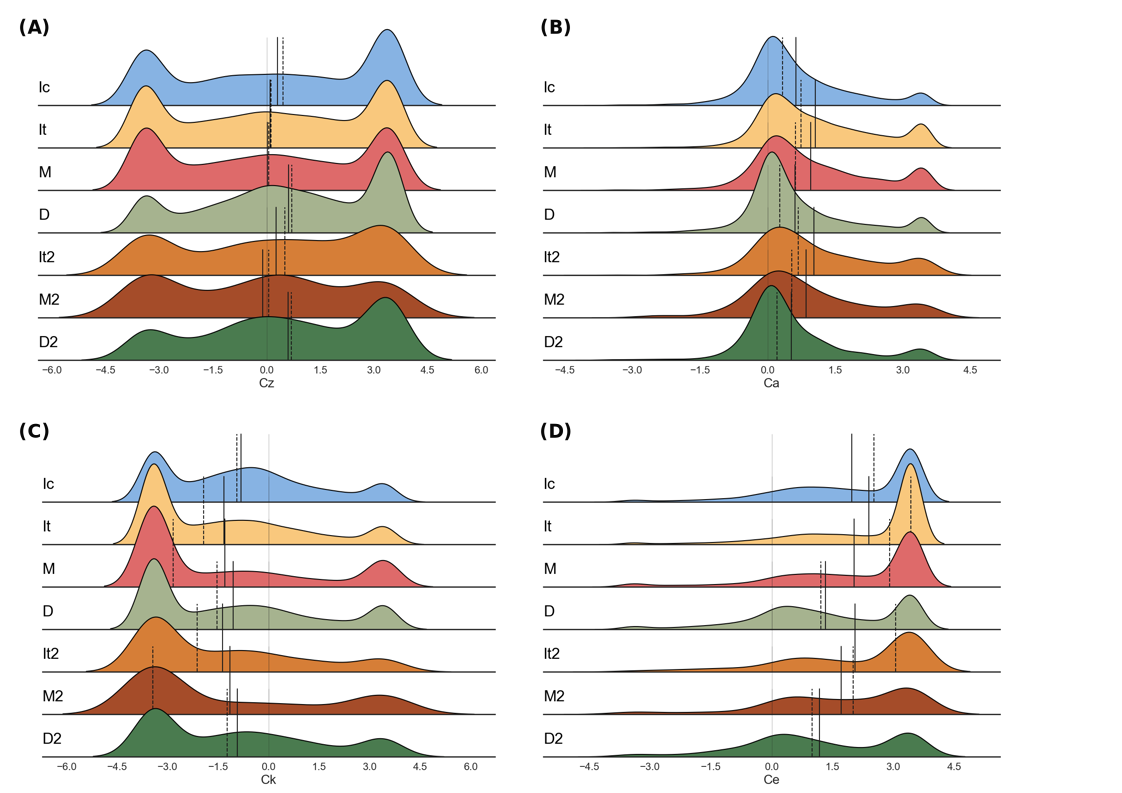
\includegraphics[width=\textwidth]{figs_5/ridge_plot_Conversion Terms.pdf}
\caption[Density Plots - Energy Terms]{Density plots for conversion terms $C_Z$ (A), $C_A$ (B), $C_K$ (C), and $C_R$ (D), for each development phase: incipient (Ic), intensification (It), mature (M), decay (D) and the secondary development phases (indicated by "2"). The solid vertical lines indicate the mean values for a given phase while the dashed lines, the median values. The units are $W m^{-2}$.}
\label{fig:ridge_plot_Conversion}
\end{figure}

The $C_Z$ term exhibits high variability in its density distribution across the different development phases (Figure \ref{fig:ridge_plot_Conversion}a). During the incipient phase, there are two distinct peaks: one at negative values and a sharper peak at positive values, with a broad distribution in between, resulting in positive mean and median values. In contrast, the intensification and mature phases display symmetric peaks at both ends of the spectrum, with a broader peak at neutral values. For the decay phase, the peak at negative values diminishes, while the peaks at neutral and positive values become sharper, pushing the mean and median to positive values. The second intensification phase, despite having peaks at neutral, positive, and negative values, shows a wide distribution in the positive range, reflected in its positive mean and median values. Lastly, the second mature and decay phases present opposite shapes: the former has a sharper peak at negative values, while the latter has a sharper peak at positive values. For the second mature phase, the mean and median values are on opposite sides of the spectrum. Therefore, while the initial and final phases of each development cycle tend to have overall positive values and the intermediate phases tend toward neutrality, the high variability makes it difficult to define a definitive behavior for the $C_Z$ term. This high variability (across systems and phases) is also noted in previous studies \citep[e.g.]{michaelides1987limited,veiga2008analysis,dias2011energy,dias2013synoptic}.

For the $C_A$ term, each phase presents a peak near neutral values, right-skewed with a long tail distribution extending towards positive values (Figure \ref{fig:ridge_plot_Conversion}b). There are also a minor peaks near $3 W s^{-2}$, which are sharper for the phases of the first development cycle. Furthermore, the distributions become more right-skewed in the intensification phases (1 and 2) and less skewed in the later phases. Consequently, the mean and median values increase from the beginning of each development cycle, peak during each intensification phase, and then decrease afterward. This indicates an overall tendency for energy to be converted from $A_Z$ to $A_E$ during the development cycle, which aligns with the overall trend observed for the $A_E$ term (Figure \ref{fig:ridge_plot_Energy}b).

The $C_K$ term, across all phases, presents a peak at negative values, right-skewed towards positive values with a minor peak at positive values (Figure \ref{fig:ridge_plot_Conversion}c). During the first development cycle, the incipient stage shows a sharp peak near $-3.5 W s^{-2}$ and a minor peak near $-1 W s^{-2}$. As the systems intensify, the minor peak becomes broader and the sharp peak becomes more pronounced. Meanwhile, the peak at positive values, near $3.5 W s^{-2}$, also becomes sharper. Consequently, the median values become significantly more negative from the incipient to the mature phase and less negative during the decay phase. Although the mean values follow a similar pattern, the sharper peak at positive values during the mature phase results in mean values for the mature phase that are similar to — or even less negative than — those of the intensification phase. The secondary development cycle shows a similar behavior to the first one. These results indicate an overall tendency for conversion from $K_Z$ to $K_E$ throughout the cyclone's life cycle, but with a significant number of systems where the energy flows in the opposite direction. The tendency for $C_K$ to be negative and most intense during mature phases is consistent with the overall behavior of the $K_E$ term. However, this analysis does not clarify whether there are instances where the energy flow reverses direction during the life cycle. This will be investigated in the next sections, as previous studies have suggested that such reversals might occur, especially in systems transitioning from one type to another \citep[e.g.,]{brennan1980zonal,michaelides1987limited,wahab2002mechanism,veiga2008analysis,pezza2010environmental}.

The density distributions for all phases of the $C_E$ term present peaks at positive values, near $3.5 W s^{-2}$, with left-skewed distributions and long tails extending into negative values, albeit with low densities (Figure \ref{fig:ridge_plot_Conversion}d). The peaks tend to become sharper during the intensification phases and decrease afterward. Additionally, for the decay phases (1 and 2), a broad peak near neutral values emerges. As a result, the mean and median values are higher during the intensification phases and closer to zero during the decay phases (1 and 2). Since the peaks in conversion from $A_E$ to $K_E$ coincide with the phases where $A_E$ is on average highest, it can be inferred that a significant amount of the energy content in this term is being converted to $K_E$.

The density plots for the boundary terms are displayed in Figure \ref{fig:ridge_plot_Boundary}. The $BA_Z$ term presents a right-skewed distribution peaking at values close to zero (Figure \ref{fig:ridge_plot_Boundary}a). There are also long tail distributions towards high positive values, indicating the occurrence of unusually extreme values. This behavior is reflected in the overall positive mean and median values. Across the phases, there is a tendency for the imports of $A_Z$ to decrease from the intensification to mature phases (1 and 2), increasing again for the decay phases (1 and 2). This behavior is consistent with the values for the $A_Z$ term (Figure \ref{fig:ridge_plot_Energy}).

\begin{figure}[!htbp]
\centering
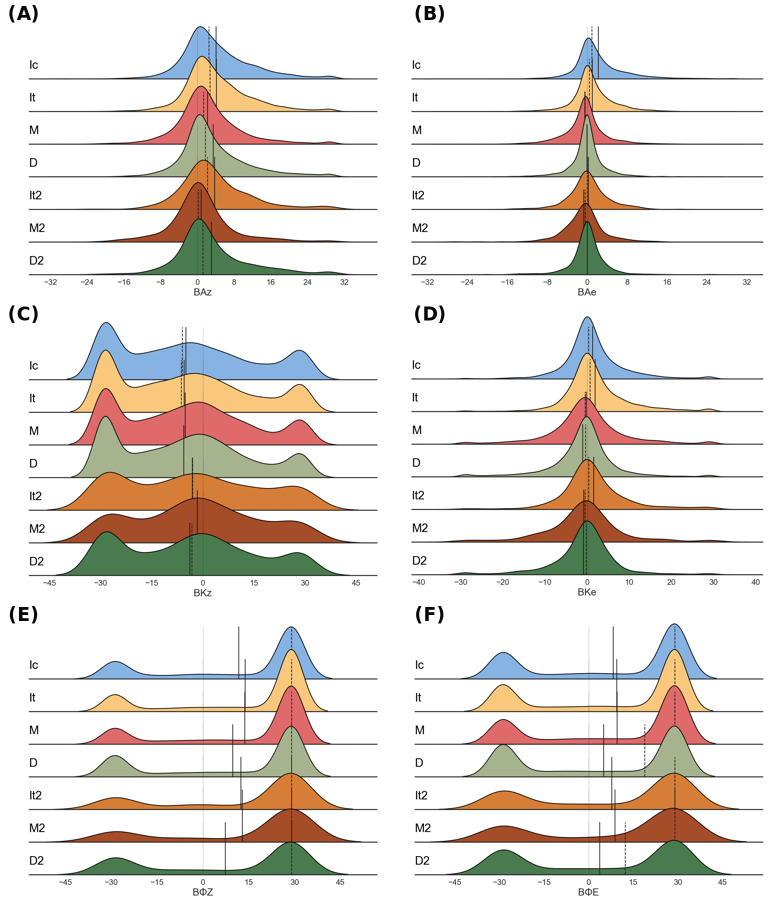
\includegraphics[width=\textwidth]{figs_5/ridge_plot_Boundary Terms.pdf}
\caption[Density Plots - Energy Terms]{Density plots for boundary terms $BA_Z$ (A), $BA_E$ (B), $BK_Z$ (C), $BK_E$ (D) and boundary pressure work terms $B\Phi Z$ and $B\Phi E$, for each development phase: incipient (Ic), intensification (It), mature (M), decay (D) and the secondary development phases (indicated by "2"). The solid vertical lines indicate the mean values for a given phase while the dashed lines, the median values. The units are $W m^{-2}$.}
\label{fig:ridge_plot_Boundary}
\end{figure}

The $BA_E$ and $BK_E$ terms present similar distributions, with sharp peaks near zero and long tails extending towards both negative and, especially, positive values (Figures \ref{fig:ridge_plot_Boundary}b and \ref{fig:ridge_plot_Boundary}d). Consequently, the mean and median values are often positive. Despite the similarities in the density distributions, the overall behavior across the distinct phases among these terms differs. For $BA_E$, there is a tendency for the mean and median values to decrease from the beginning of each development cycle to the mature phase, becoming negative in the latter and increasing again during decay, but with mean and median values near zero. This behavior indicates imports of $A_E$ in the systems' early life stages but exports as they mature. Meanwhile, for $BK_E$, the mean and median values tend to increase from the incipient to the intensification phases and then decrease from the intensification (1 and 2) to the decay phases (1 and 2), displaying negative mean and median values at the mature and decay phases. This indicates that after intensification, the systems overall export $K_E$ outside the computational domain.

The $BK_Z$ term presents densities peaking at positive, neutral, and negative values (Figure \ref{fig:ridge_plot_Boundary}c). Across all phases, the peaks are often sharpest at negative values, but the peaks at neutral values tend to become sharper throughout the systems' life cycles. The mean and median values are similar for the first development cycle phases, while the differences are more marked for the second development cycle phases, with mean and median values becoming more positive from intensification 2 to mature 2 and then decreasing in the decay 2 phase. Overall, this pattern indicates a tendency for systems to consistently export $K_Z$ through their life cycles, although there is significant variability in the data.

Lastly, $B\Phi Z$ and $B\Phi E$ display nearly identical distributions, presenting peaks at both positive and negative values, but with sharper peaks at the former (Figures \ref{fig:ridge_plot_Boundary}e and \ref{fig:ridge_plot_Boundary}f). As a result, the median values are often aligned across all phases in the positive range. However, during the decay phase, the peaks at negative values become sharper, especially for $B\Phi E$, which causes the median values to decrease. As discussed in Section \ref{math}, the physical interpretation of these terms is difficult and can be hindered by small errors in the geopotential field, which might lead to unusually high values.

Figure \ref{fig:ridge_plot_Generation} displays the densities for the generation and the residuals of the dissipation terms. Here, the generation terms will be explored instead of their residuals as they allow for a physical interpretation, while the residuals account for numerical errors that escalate from the other terms in the $A_Z$ and $A_E$ budgets. For the $G_Z$ term, each phase often displays distributions with peaks at neutral values and minor peaks at positive and negative values (Figure \ref{fig:ridge_plot_Generation}a). During the incipient stage, the peak at neutral values is broader, resulting in negative mean and median values. As the systems evolve, the peak at neutral values becomes sharper, causing the mean and median values to approach zero by the decay phase. Notably, for the second mature phase, the minor peak at positive values diminishes, causing the mean and median values to become negative again.

\begin{figure}[!htbp]
\centering
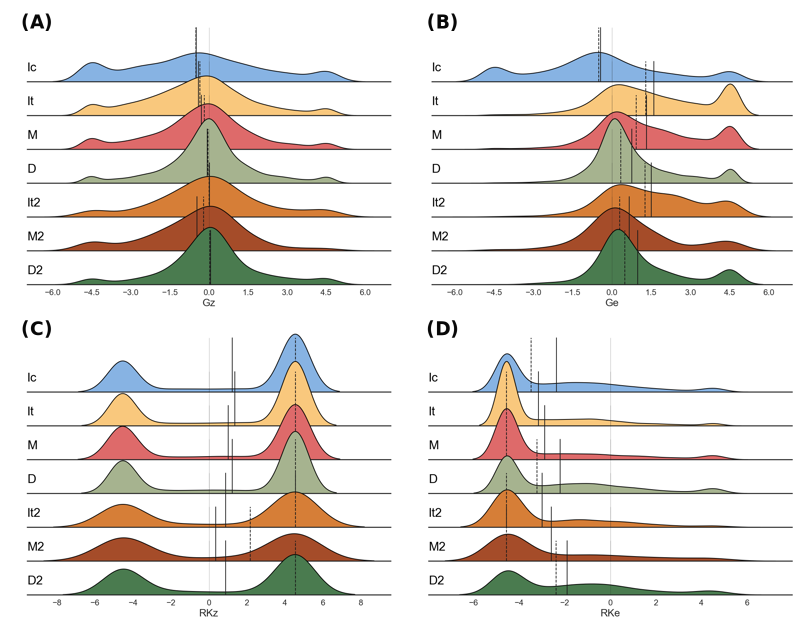
\includegraphics[width=\textwidth]{figs_5/ridge_plot_Generation and Dissipation Terms.pdf}
\caption[Density Plots - Energy Terms]{Density plots for generation and dissipation residual terms $G_Z$ (A), $G_E$ (B), $RK_Z$ (C), and $RK_E$ (D), for each development phase: incipient (Ic), intensification (It), mature (M), decay (D) and the secondary development phases (indicated by "2"). The solid vertical lines indicate the mean values for a given phase while the dashed lines, the median values. The units are $W m^{-2}$.}
\label{fig:ridge_plot_Generation}
\end{figure}

Surprisingly, the $G_E$ term presents an identical distribution to the $G_Z$ term for the incipient phase, while the other phases display peaks at both neutral and positive values, with high inter-phase variability (Figure \ref{fig:ridge_plot_Generation}b). During the intensification phase, there is a broad right-skewed peak at neutral values, followed by a sharper peak at positive values. As the systems transition to the mature and decay phases, the peak at positive values decreases and the peak at neutral values becomes broader. Overall, there are negative mean and median values during the incipient stage, reaching the largest positive values in the intensification phase and decreasing through the mature and decay phases. The second development cycle, in turn, presents a distinctive behavior: while the values are largest for intensification 2 and decrease during the mature 2 phase, they increase again during the decay 2 phase. Overall, these results indicate a generation of $A_E$ especially during the intensification phases, which decreases afterward, consistent with the overall $A_E$ behavior (Figure \ref{fig:ridge_plot_Energy}).

The $RK_Z$ term displays distributions with peaks at both negative and positive values, but with small inter-phase variability, similar to the $B\Phi Z$ term (Figure \ref{fig:ridge_plot_Generation}c). This suggests an influence of the latter on the former term, although the magnitudes are much smaller. Due to the sharper peak at positive values compared to the one at negative values, the mean and median values are positive across all phases, with median values being identical. Meanwhile, $RK_E$ presents right-skewed peaks at negative values, with long tail distributions extending towards positive values (Figure \ref{fig:ridge_plot_Generation}d). The mean and median values for this term increase from the intensification to decay phases. Although it is tempting to associate the positive values of $RK_Z$ with either the upscaling of energy and generation of $K_Z$ through zonal jet fluxes towards the low-pressure system, and the negative values of both $RK_Z$ and $RK_E$ with kinetic energy dissipation, the assimilation of numerical errors and boundary pressure work terms prevents drawing such conclusions.

Finally, the budget terms result from the aggregate contributions of each energy cycle term. The density distributions for these terms are illustrated in Figure \ref{fig:ridge_plot_Budget}. Due to the high variability often present in each individual term, the budget terms also exhibit high variability, with modest inter-phase variations in shape distribution (i.e., although the overall behavior is preserved among the distinct phases, the magnitude of the peaks changes).

\begin{figure}[!htbp]
\centering
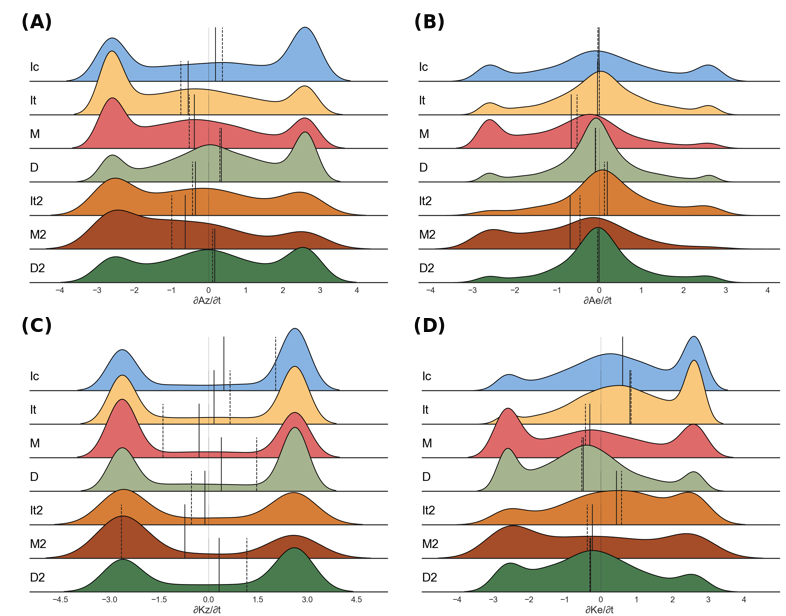
\includegraphics[width=\textwidth]{figs_5/ridge_plot_Budget Terms.pdf}
\caption[Density Plots - Energy Terms]{Density plots for energy budget terms $\frac{\partial A_Z}{\partial t}$ (A), $\frac{\partial A_E}{\partial t}$ (B), $\frac{\partial K_Z}{\partial t}$ (C), and $\frac{\partial K_E}{\partial t}$ (D), for each development phase: incipient (Ic), intensification (It), mature (M), decay (D) and the secondary development phases (indicated by "2"). The solid vertical lines indicate the mean values for a given phase while the dashed lines, the median values. The units are $W m^{-2}$.}
\label{fig:ridge_plot_Budget}
\end{figure}

The $\frac{\partial A_Z}{\partial t}$ term often presents three peaks across the distinct phases: one at positive, negative, and neutral values (Figure \ref{fig:ridge_plot_Budget}a). For the incipient phase, the peak at positive values is more prominent, while for the intensification and mature phases, the peak at negative values is more significant. The decay phase displays an increase in the peaks at neutral and positive values. A similar behavior is seen for the secondary development phases. As indicated by the mean and median values, $A_Z$ usually increases during incipient and decay phases, displaying decreases during the other phases.

Meanwhile, the $\frac{\partial A_E}{\partial t}$ term often displays a sharp peak at neutral values, with long tail distributions towards both positive and negative values. The exceptions are the mature phases (1 and 2), which are left-skewed and present broad peaks at negative values. As a result, while most phases tend towards neutrality for the $A_E$ term, the mature phases tend to decrease this term.

For the $\frac{\partial K_Z}{\partial t}$ term, a distribution with peaks at opposite sides of the spectrum can be seen (Figure \ref{fig:ridge_plot_Budget}c). The differences among each phase lie in the positioning of the sharpest peak. Overall, for the first development cycle, there is a tendency for $K_Z$ to increase over the incipient and intensification phases, decrease during the mature phase, and then increase again during the decay phase. Despite the tendency for decreases during the second intensification, the peaks at each end of the spectrum are nearly symmetrical. The second mature phase presents an overall tendency for decreases in $K_Z$, which is reversed during the second decay. These results suggest that $K_E$ is often increasing or decreasing but rarely neutral, and despite the overall trends noted here, there is high variability in behavior among the systems.

Lastly, for $\frac{\partial K_E}{\partial t}$, the distributions present peaks at positive, neutral, and negative values, with large inter-phase differences (Figure \ref{fig:ridge_plot_Budget}d). For the incipient and intensification phases, the peaks are sharper at positive values, which is reversed during the mature and decay phases. This behavior is reflected in the mean and median values. A similar behavior can be noted for the secondary development phases. These results indicate a tendency for $K_E$ to increase during its initial development for each cycle, peaking during the intensification phases (1 and 2), while the tendency in subsequent phases is a decrease.

\subsection{Mean Energy Cycle}\label{sec:lec_mean_phases}

Figure \ref{fig:lec_mean_values_phases} illustrates the LEC for the mean values of each term for the first development cycle. As noted in Section \ref{sec:climatological_aspects}, due to the high variability presented for the distinct terms, the results should be interpreted with caution. However, they can provide an overview of the mean energy fluxes in the analyzed systems across the different development phases and their respective dynamical evolution. Additionally, similarly to Figure \ref{fig:lec_mean_values}, the $G_Z$ and $G_E$ terms are used instead of their respective residuals for a more physically based interpretation, although the budgets were computed using the residuals. Since the residual terms were integrated into the budgets, the presented budgets may not perfectly balance positive and negative energy fluxes due to the finite differences method used, which also incorporates numerical errors.

\begin{figure}[!htbp]
\centering
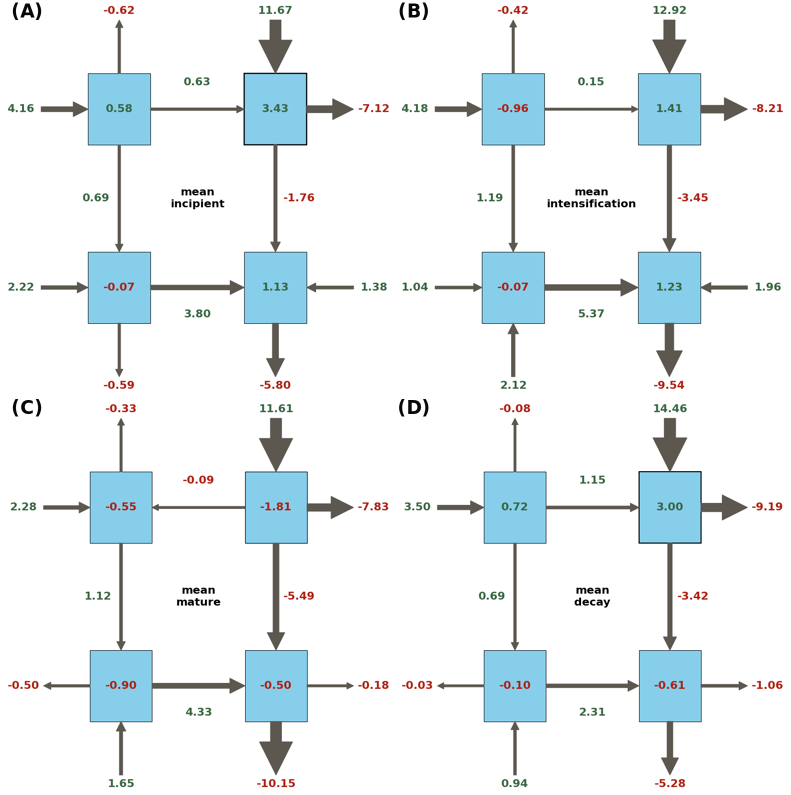
\includegraphics[width=\textwidth]{figs_5/lec_mean_values_phases.pdf}
\caption[LEC - Mean Life Cycle for Each Phase]{Mean values of the Lorenz Energy Cycle (LEC) terms for each life cycle phase: incipient (A), intensification (B), mature (C), and decay (D). Each blue box represents an energy component, with arrows showing the direction of energy flow. The numbers adjacent to the arrows indicate the magnitude and direction of the energy flux, with green indicating positive values and red indicating negative values. A representation of the complete cycle, with the positioning of each term can be found at Figure \ref{fig:lec_mean_values}.}
\label{fig:lec_mean_values_phases}
\end{figure}

The incipient stage is confirmed as the development stage where the cyclone is not fully formed and the eddy-related environmental energetics are still responding to large-scale dynamics. This is mostly indicated by the $A_Z$ term, which is increasing due to heating at low latitudes and diabatic cooling at higher latitudes. However, this increase is not driven by $G_Z$, but rather from imports of $A_Z$. Such behavior (both $G_Z < 0$ and $BA_Z > 0$) has been observed in study cases, but often the $\frac{\partial A_Z}{\partial t}$ is negative in the initial phases \citep[e.g.,]{brennan1980zonal,dias2011energy,dias2013synoptic}. The excess $A_Z$ is being converted into both $K_Z$ and $A_E$ as, in this phase, while a meridional temperature gradient is still present, there are also eddy meridional heat transports.

The $K_Z$ term experiences the largest increases during this phase, driven mainly by $RK_Z$, although a significant portion of this energy is exported outside the domain, with some of it converted to $K_E$. In contrast, $A_E$ experiences modest decreases. The negative $\frac{\partial A_E}{\partial t}$ indicates that the initial $A_E$ reservoir must be large enough to sustain the eddy development. As Figure \ref{fig:ridge_plot_Energy} demonstrated, this is indeed the case. The existence of a zonal temperature gradient drives the conversion of $A_E$ into $K_E$. This initial conversion chain of $A_Z \rightarrow K_Z$ and $A_Z \rightarrow A_E \rightarrow K_E$ is observed in the initial stages of most LECs of baroclinic disturbances previously reported \citep[e.g.,]{michaelides1992spatial,pezza2010environmental,dias2011energy,black2013universal}.

While $A_E$ receives energy from $A_Z$ and there are some imports of $A_E$ through the boundaries, this energy is mostly converted to $K_E$. Additionally, during this stage, $G_E$ is negative, possibly due to the lower convective activity at the cyclone's initial development. The $K_E$ term then experiences increases in energy, driven by the barotropic conversion term, imports of energy, and mainly conversions from $A_E$, although a significant portion of this energy is lost through $RK_E$.

During the intensification phase, although the loss of $A_Z$ energy from the $G_Z$ term and the conversion to $K_Z$ diminish, the enhancement in conversion to $A_E$ causes an overall decrease in this term. This indicates a weakening of the meridional temperature gradient, driven by the eddy-induced meridional heat transport. For the $K_Z$ term, the enhanced $RK_Z$ is balanced by increased export of energy and conversion to $K_E$, leading to a decrease in the magnitude of $\frac{\partial K_Z}{\partial t}$.

In this phase, enhanced eddy-related convective processes are evident, indicated by the positive $G_E$. This process, in conjunction with the increased meridional heat transport, creates zonal temperature and $\omega$ gradients, enhancing $A_E \rightarrow K_E$ conversions. With reduced $A_E$ imports, the magnitude of $\frac{\partial A_E}{\partial t}$ remains consistent with the incipient phase. For the $K_E$ term, despite increases in all energy influxes, the increased activity of $RK_E$ results in only modest increments in $\frac{\partial K_E}{\partial t}$.

In the mature phase, most LEC terms present an overall reduction in magnitude as the system's energetics become less active and begin to equalize with the environment. The exception is the barotropic term $C_K$, which increases in magnitude. As a result, the $K_Z$ term begins to experience decreases, indicating an overall weakening of the zonal jets. The $\frac{\partial A_E}{\partial t}$ term becomes significantly more negative, primarily due to the reduction in convective activity, as indicated by the $G_E$ term, and because this term starts to export energy outside the domain.

The $\frac{\partial K_E}{\partial t}$ term also experiences decreases, presenting a reversal in sign, despite the enhanced barotropic conversions ($C_K$ term), indicating a weakening of the eddy activity. This is due to the combined effect of the reduced conversion from $A_E$ — indicating an overall reduction in zonal temperature gradients — and the reversal in sign of $BK_E$, as the eddy begins to export energy outside the domain, alongside further increases in the magnitude of the $RK_E$ term.

Lastly, in the decay phase following the mature phase, most terms present a further overall reduction in magnitude. The $\frac{\partial A_Z}{\partial t}$ reverts to its original positive values, driven by the enhanced imports of energy. A similar behavior is observed for $\frac{\partial K_Z}{\partial t}$, presenting comparable magnitudes to their values during the incipient phase. This scenario suggests that as the eddy decays, the atmosphere regains its original behavior, with the equator-to-pole temperature gradients increasing and the zonal jets strengthening.

The $\frac{\partial A_E}{\partial t}$ term also presents a magnitude comparable to the incipient stage. However, the $A_E$ boundary and generation terms present opposite signs during the decay phase compared to the incipient phase, with $G_E$ being positive due to residual convective activity, although less vigorous than in previous phases, and minimal exports of $A_E$ through the boundaries. Despite the decrease in magnitude of $RK_E$, the reduced contributions from $C_E$ — due to weakened zonal gradients — and $C_K$ — due to reduced barotropic conversions — along with the enhanced export of energy, result in the $K_E$ term presenting its largest decreases across all phases.

Notably, the energy fluxes often maintain the same direction across all development phases, although the terms exhibit notable variations in magnitude. For instance, both the baroclinic chain and the barotropic conversion term are active throughout the entire life cycle. For baroclinic disturbances, this consistency in the baroclinic chain is expected \citep[e.g.,]{pezza2010environmental,dias2011energy,black2013universal}, although high variability is present and this behavior can vary from case to case (Figure \ref{fig:ridge_plot_Conversion}). Regarding barotropic conversions, some studies report its predominance in extratropical cyclone development \citep[e.g.,]{michaelides1987limited,wahab2002mechanism,bulic2006limited,cavicchia2018energetics}, while others do not \citep[e.g.,]{pezza2010environmental,dias2011energy}. Here, it is believed that the choice of computational domain as well as the use of a Semi-Lagrangian framework might aid in making barotropic conversions more evident \citep{michaelides1999quasi}. The next sections will explore this more deeply.

The contributions from $G_E$ are negative during the incipient phase, peaking during intensification, and diminishing afterward, which is consistent with previous studies \citep[e.g.,]{michaelides1987limited,dias2011energy,wahab2002mechanism}, although those studies analyze the $RG_E$ term, making direct comparisons difficult. While the moist baroclinic chain is most intense during the intensification phase, the barotropic conversion is most intense during the mature phase. The $RK_Z$ and $RK_E$ terms are also consistent across all phases: $RK_Z$ provides energy to $K_Z$, while $RK_E$ acts as a sink of energy. Although both residuals aggregate a combination of terms, making it difficult to attribute the overall behavior to a specific term, the results presented here align with \citet{smith1980energetics}, which indicated high generation of kinetic energy by cross-contour flow and high dissipation of $K_E$ throughout the system's life cycle. Moreover, the overall paradox related to the negative sign of the term $\frac{\partial A_E}{\partial t}$ might be attributed to the inclusion of numerical errors in the energy budget.

Figure \ref{fig:lec_mean_values_phases_second} displays the Lorenz Energy Cycle (LEC) for the mean values of each term for the second development cycle. The overall energy flux for each LEC term remains the same as for the first development cycle: the baroclinic chain is most active during the second intensification phase, while the barotropic conversion term is most active during the second mature phase, along with higher $RK_E$. Notably, the $\frac{\partial A_E}{\partial t}$ term presents positive values during the second intensification, while, for the same phase, the $RK_Z$ shows its lowest values and $C_K$ its highest values across all phases. Furthermore, the values of $C_A$ and $C_E$ are lower than their respective counterparts in the first development cycle. These results suggest that distinct dynamical processes are related to the development during the second cycle.

\begin{figure}[!htbp]
\centering
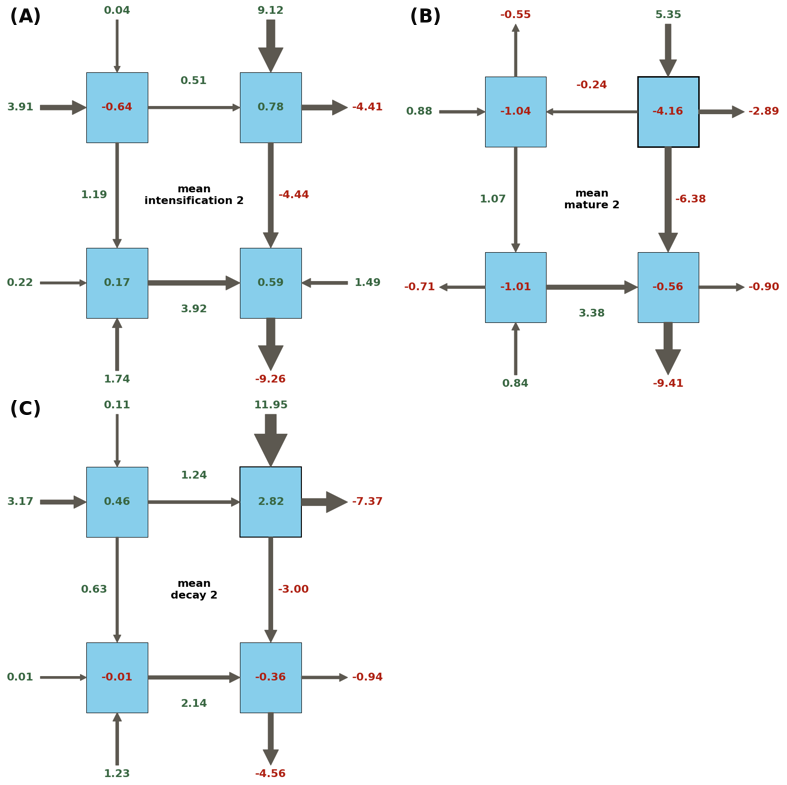
\includegraphics[width=\textwidth]{figs_5/lec_mean_values_phases_second.pdf}
\caption[LEC - Mean Life Cycle for Each Phase]{Mean values of the Lorenz Energy Cycle (LEC) terms for each phase of the cyclones secondary development: intensification 2 (A), mature 2 (B), and decay 2 (C). Each blue box represents an energy component, with arrows showing the direction of energy flow. The numbers adjacent to the arrows indicate the magnitude and direction of the energy flux, with green indicating positive values and red indicating negative values. A representation of the complete cycle, with the positioning of each term can be found at Figure \ref{fig:lec_mean_values}.}
\label{fig:lec_mean_values_phases_second}
\end{figure}

The analysis of the LEC across different development phases reveals significant insights into the energy dynamics of cyclonic systems. During the incipient phase, there is a notable increase in $A_Z$, primarily due to imports rather than generation, with conversions to $K_Z$ and $A_E$ occurring. The intensification phase sees enhanced eddy-related convective processes and thermally direct circulation, leading to increased conversions from $A_E$ to $K_E$. The mature phase is characterized by a reduction in overall energy magnitudes and a weakening of zonal jets. In the decay phase, the system's energetics further diminish, suggesting a reversion to the atmosphere's original state.

The second development cycle exhibits similar energy flux patterns, with distinct variations in the intensity of key energy fluxes, indicating an enhanced importance of barotropic conversions. These findings underscore the importance of both baroclinic and barotropic processes in different phases. The baroclinic chain is especially important during the intensification phase, consistent with previous studies on extratropical cyclone development, while barotropic conversions become more evident in the mature phase and in the secondary development cycle. The observed high variability and the integration of residual terms into the budgets suggest that numerical errors and domain choices significantly influence the interpretation of these energy cycles.

\subsection{EOFs}\label{sec:eof_phases}


Similar to the mean behavior presented in Section \ref{sec:lec_mean}, the results for the mean behavior across each life phase exhibit high variability. Therefore, each term can span a wide range of possible values, possibly resulting in reversals of energy fluxes. To delineate an overall picture of the LEC across each phase for cyclones in the SESA region, unlike the presentation in Section \ref{fig:eofs_total}, the reconstructed EOFs will be analyzed. These were computed by reversing the normalization process and adding back the mean to each EOF. Here, the analysis is limited to the first developmental cycle for simplicity, justified by the higher prevalence of systems that only present one developmental cycle.

Figure \ref{fig:variance_explained_all_phases} illustrates the proportion of variance in the dataset that is explained by each of the first four Empirical Orthogonal Functions (EOFs) for each life phase. As shown for the EOFs representing the mean LEC behavior, the first four EOFs explain the main modes of variability contained in the data. For practical reasons, only the first four EOFs will be explored. Similar to the total life cycle, the first EOF accounts for the largest portion of the variance for all phases, explaining approximately 26\% to 30\%, indicating it captures the most significant pattern in the data. The exception is the incipient phase, where EOF1 explains approximately 21\% of the variance in the data. Meanwhile, the subsequent EOFs explain progressively smaller proportions of the variance. Furthermore, as discussed in Section \ref{fig:eofs_total}, the PCs will not be presented as they would merely represent the signal magnitude across the distinct cyclones rather than any physical feature.

\begin{figure}[!htbp]
\centering
\includegraphics[width=\textwidth]{figs_5/variance_explained_all_phases.png}
\caption[EOF - Explained Variance for Each Phase]{Proportion of variance in the dataset explained by the first four Empirical Orthogonal Functions (EOFs), for each development phase.}
\label{fig:variance_explained_all_phases}
\end{figure}

For EOF1 (Figure \ref{fig:eof1_phases}), most terms reinforce the overall behavior presented for the mean values across each phase (Figure \ref{fig:lec_mean_values_phases}). An enhancement of both the baroclinic chain and the barotropic conversion from $K_Z$ to $K_E$ is consistent across all phases. Both instabilities increase in activity during the life cycle, decreasing at the onset of the decay phase: the baroclinic chain presents higher values during the incipient phase and peaks during the intensification phase, while the barotropic conversion peaks during the mature phase. Notably, the $G_E$ term is enhanced and positive throughout all phases, peaking during intensification, indicating overall enhanced convective activity for this EOF.

Furthermore, $RK_Z$ is highly enhanced, resulting in positive tendencies for $\frac{\partial K_Z}{\partial t}$. However, this positive tendency is not significantly above the average, as most of the excess energy is exported outside the domain via the $BK_Z$ term. A similar behavior is found for $\frac{\partial K_E}{\partial t}$. Despite the increased energy influxes for $K_E$, they are accompanied by significant increases in $RK_E$, which sinks that extra energy. Additionally, despite the enhanced imports of $K_E$ during the incipient and intensification phases, the mature and decay phases observe enhanced exports.

Other distinctions from the mean behavior are found in the budgets for $A_Z$ and $A_E$ terms. For $A_Z$, there is a negative tendency during the incipient phase, indicating a weakening of the meridional temperature gradients during the cyclone's initial development. Meanwhile, for the $A_E$ budget, an enhancement above the mean conditions is observed, resulting in a positive budget for the incipient and intensification phases. This indicates that the negative values found in the mean behavior might be attributed to the presence of outliers.

\begin{figure}[!htbp]
\centering
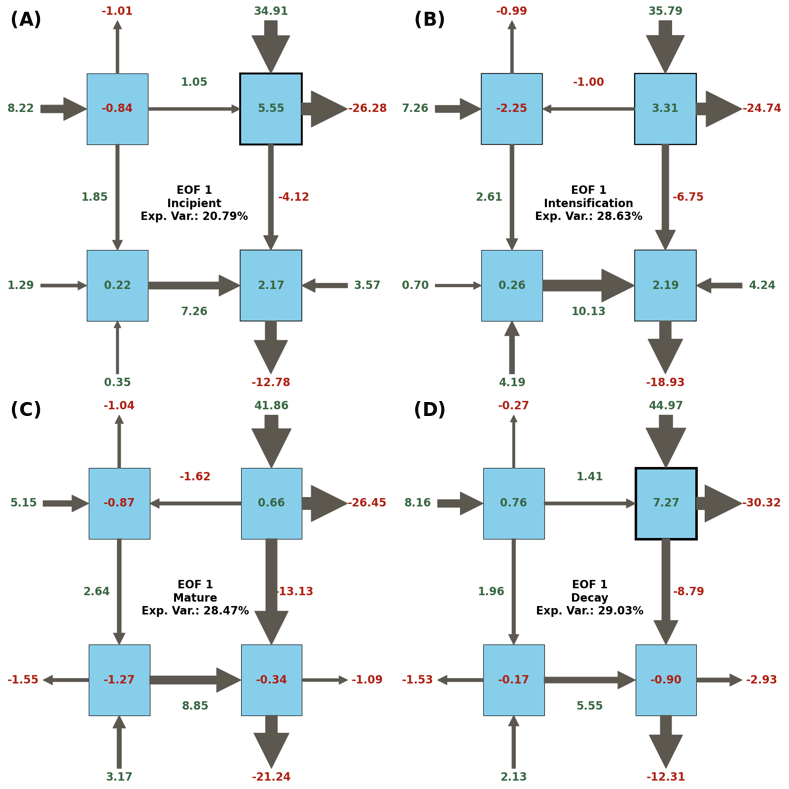
\includegraphics[width=\textwidth]{figs_5/eof1_phases_reconstructed.pdf}
\caption[Reconstructed EOF1 - Phases]{Reconstructed first EOF (EOF1) of Lorenz Energy Cycle (LEC) Terms, illustrating energy fluxes across each phase of the first development cycle: incipient (A), intensification (B), mature (C) and decay (D).  The numbers adjacent to the arrows denote the magnitude and direction of the anomaly, with green indicating positive values and red indicating negative values.}
\label{fig:eof1_phases}
\end{figure}

In EOF2, the overall mean behavior is weakened for most terms (Figure \ref{fig:eof2_phases}). Notably, during the incipient stage, there is a deviation in the energy flux from $K_Z$: a reversal in the sign of the $C_Z$ term and a reduction in barotropic conversions are observed. The negative $C_Z$, accompanied by negative $G_Z$ and positive $C_A$, indicates an overall weakening of the meridional gradient in vertical motions. During this stage, there is also a stronger than average negative $G_E$ but a strengthening of $C_E$, which is explained by imports of $A_E$ through the boundaries.

For the remaining phases, the import of $A_E$ reduces, the barotropic conversion progressively increases, and the $G_E$ term is similar to the mean behavior. Despite this, $\frac{\partial K_E}{\partial t}$ presents a below-average tendency. This can be explained by the enhancement of sinks via the $RK_E$ term during the intensification and mature phases, and the progressively increased exports of $K_E$. During the decay phase, although the sink from the $RK_E$ term reduces significantly while $C_K$ is strongest, this is compensated by the highest exports of energy and the weakest conversions from $A_E$.

Furthermore, from the intensification phase onwards, an enhancement of $RK_Z$ can be seen, which, similar to EOF1, is followed by an enhancement of exports of $K_Z$. During the decay phase, $\frac{\partial A_Z}{\partial t}$ presents significant increases, followed by a reversal in the sign of $C_Z$ compared to previous states. These combined processes result in an enhancement of $\frac{\partial K_Z}{\partial t}$, making it twice the average mean.


\begin{figure}[!htbp]
\centering
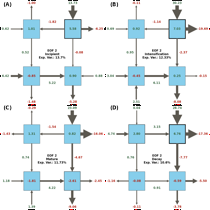
\includegraphics[width=\textwidth]{figs_5/eof2_phases_reconstructed.pdf}
\caption[Reconstructed EOF2 - Phases]{Reconstructed second EOF (EOF2) of Lorenz Energy Cycle (LEC) Terms, illustrating energy fluxes across each phase of the first development cycle: incipient (A), intensification (B), mature (C) and decay (D).  The numbers adjacent to the arrows denote the magnitude and direction of the anomaly, with green indicating positive values and red indicating negative values.}
\label{fig:eof2_phases}
\end{figure}

For EOF3, the inter-phase variability is less marked (Figure \ref{fig:eof3_phases}). Across all phases, there are high values of $RK_Z$, which — similarly to the previous EOFs — are almost compensated by exports of $K_Z$. There is also a consistent conversion from $A_Z$ to $K_Z$ and imports of $A_Z$. During the incipient phase, positive $\frac{\partial A_Z}{\partial t}$ is found due to the importation of energy and positive generation ($G_Z$). There is then a conversion of $A_Z$ into $A_E$ and $K_Z$. $\frac{\partial A_Z}{\partial t}$ is unusually high due to the enhanced $RK_Z$ and thus provides above-average energy to $K_E$. Meanwhile, $\frac{\partial A_E}{\partial t}$ is increasing — due to the combined effects of $C_A$, imports, and enhanced convective activity — and is providing energy to $K_E$. This term, in turn, is exporting energy and losing it via $RK_E$. During the intensification and mature phases, the imports of $A_E$ become exports of energy, while the barotropic conversion becomes the highest contributor to $K_E$. Meanwhile, the $RK_E$ term peaks at the mature phase, decreasing afterward. Lastly, during the decay phase, most LEC terms are below average, indicating a weaker eddy at later stages.

\begin{figure}[!htbp]
\centering
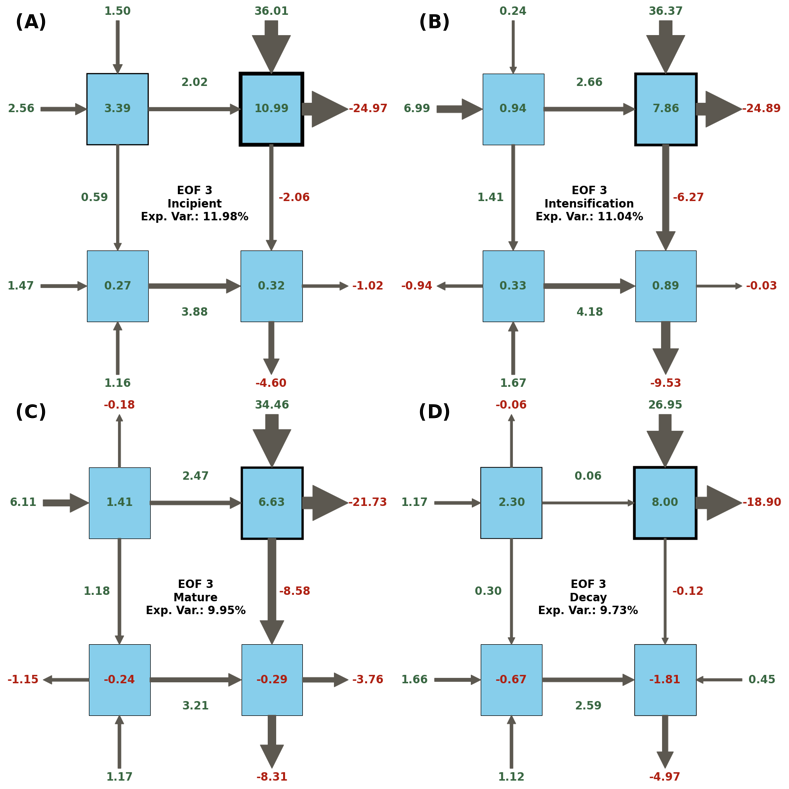
\includegraphics[width=\textwidth]{figs_5/eof3_phases_reconstructed.pdf}
\caption[Reconstructed EOF3 - Phases]{Reconstructed third EOF (EOF3) of Lorenz Energy Cycle (LEC) Terms, illustrating energy fluxes across each phase of the first development cycle: incipient (A), intensification (B), mature (C) and decay (D).  The numbers adjacent to the arrows denote the magnitude and direction of the anomaly, with green indicating positive values and red indicating negative values.}
\label{fig:eof3_phases}
\end{figure}

In EOF4, most terms generally present lower magnitudes across all phases than in the mean behavior, indicating that this EOF corresponds to weaker systems development (Figure \ref{fig:eof4_phases}). The $RK_Z$ presents above-mean values only during the incipient phase, where both $C_K$ and $C_E$ contribute equally to $K_E$. However, during this phase, $G_E$ is negative and $C_A$ is low, with the main contributor to $A_E$ being the imports of energy. As the system develops, $G_E$ becomes positive, peaking during the mature phase, and $C_A$ increases, peaking during the intensification phase. Notably, for the first time, $C_K$ is positive during the decay phase.

\begin{figure}[!htbp]
\centering
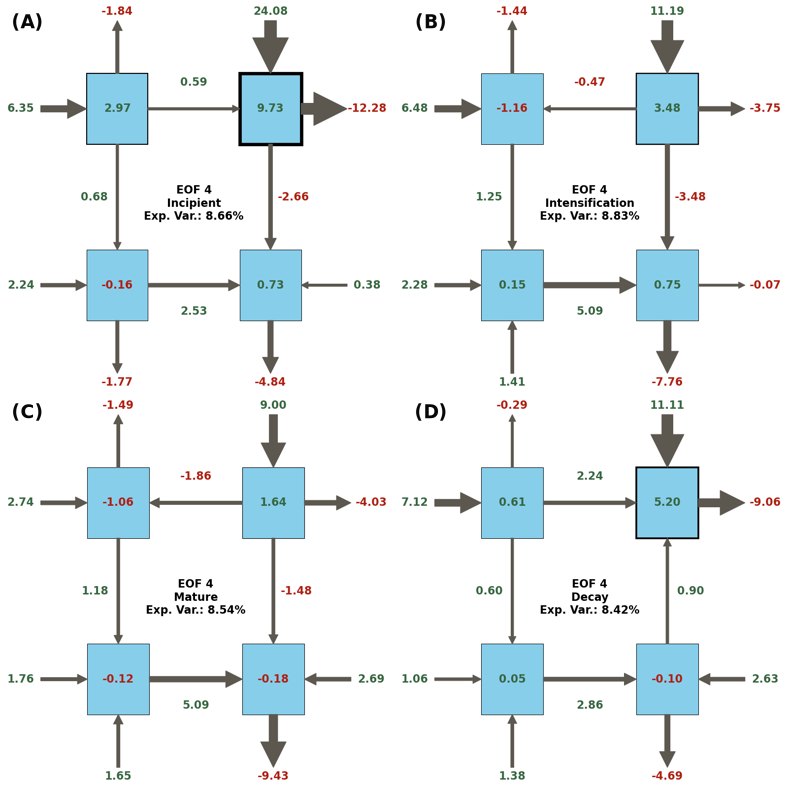
\includegraphics[width=\textwidth]{figs_5/eof4_phases_reconstructed.pdf}
\caption[Reconstructed EOF4 - Phases]{Reconstructed fourth EOF (EOF4) of Lorenz Energy Cycle (LEC) Terms, illustrating energy fluxes across each phase of the first development cycle: incipient (A), intensification (B), mature (C) and decay (D).  The numbers adjacent to the arrows denote the magnitude and direction of the anomaly, with green indicating positive values and red indicating negative values.}
\label{fig:eof4_phases}
\end{figure}

In summary, EOF1 displays a strengthening of the mean behavior — a scenario where the moist baroclinic chain and barotropic conversions sustain the eddy throughout its entire life cycle. The former is most intense during the incipient and intensification phases, while the latter is strongest during the mature and decay phases. In EOF2, cyclogenesis and initial development are triggered mostly by imports of $A_E$ and $K_E$ and the import of the former continue until the mature phase. Meanwhile, there is a consistent increase in barotropic conversions through the life cycle. In this case it seems that instead of intensifying the cyclone, the barotropic conversion acts as impeding it to decay earlier.  

For EOF3, although the initial development is fueled by the moist baroclinic chain in conjunction with imports of $A_E$, barotropic conversions dominate during the intensification and mature periods. In the decay phase, all terms are weakest. For all EOFs 1, 2, and 3, during later development stages, high barotropic conversions are typically observed. However, they are not sufficient to surpass the loss of energy from exports and the $RK_E$ term, resulting in $\frac{\partial A_E}{\partial t} < 0$. Lastly, for EOF4, while the initial development is related to imports of both $A_E$ and $K_Z$, the barotropic and especially the moist baroclinic chain lead to eddy growth. Nonetheless, the lower than average values indicate that this EOF is related to the development of weaker systems.

\section{Summary and Concluding Remarks}

This chapter delves into the energetics of cyclones in the Southwestern Atlantic, focusing on the Lorenz Energy Cycle (LEC) for 7,531 cyclonic systems originating in the ARG, LA-PLATA, and SE-BR regions. It presents the first comprehensive dataset for the South Atlantic, offering insights into the energetics of these systems over their complete life cycles and development phases. The LEC was computed using limited-area energetics through a Semi-Lagrangian approach, following the method proposed by \citet{michaelides1999quasi}. Therefore, some limitations might be recognized: the results presented represent the limited-area contributions to the global energetics \citep{smith1969contribution}, while the formulations used do not account for the displacement related to the moving domain \citep{michaelides1999quasi}. However, we advocate that by adopting the snapshot approach, where each computational domain represents a fixed domain individually, each contribution can be treated individually for each time-step. For small time-steps, the aggregate contribution would represent the evolution of the eddy environment energetics.

The results presented in this chapter demonstrate that the LEC terms exhibit high variability and many outliers, explaining the differences in results found among previous studies. The Semi-Lagrangian framework overall results in higher mean values for $K_Z$ and smaller mean $A_Z$ than those reported by previous studies. This effect is attributed to the isolation of the jet features in the domain plus the reduced meridional temperature gradients compared to when large domains are adopted. For the remaining terms, their variable behavior hinders direct comparison with the literature. However, the mean LEC behavior, presenting an overall importance of the baroclinic chain in consonance with the barotropic conversion term, corroborates previous findings.

Here, the LEC is accessed from cyclogenesis until the moment the tracking methodology stops following a given system. This moment is then considered the cyclolysis. How the environmental energetics behave pre-cyclogenesis or post-lysis remains an open question and is beyond the scope of the current study. The EOF analysis demonstrates that for both the mean behavior and across each life cycle phase, the main variability is related to the enhancement of the moist baroclinic chain and barotropic conversions from the zonal jets to the eddies. This reinforces the conclusion that the main contributions to the eddy environmental energetics come from the moist baroclinic chain in consonance with barotropic conversions. These indicate that most cyclones' life cycles are modulated by the meridional temperature gradients, which are converted into kinetic energy by eddy motion. At the same time, the cyclones are also receiving momentum from the zonal jets. This mean behavior is observed across all life phases, from cyclogenesis, often strengthened during the intensification and mature phases, and weakened during the decay. 

While these processes initiate and contribute to eddy growth, in later life stages, the $RK_E$ term and exports of $K_E$ result in the eddy's decay and dissipation. Although the $RK_E$ term also aggregates numerical errors and the $B\Phi E$ term, whose physical interpretation is not obvious, the presented results suggest that most of this term's signal is related to the dissipation of energy, which is consistent with \citet{smith1980energetics}. Nevertheless, there are also a smaller, although significant number of cases where the mechanisms leading to eddy growth are distinct, such as imports of either or both eddy forms of energy ($A_E$ and $K_E$). \citet{michaelides1999quasi} previously associated imports of $K_E$ with downstream development \citep{simmons1979downstream}, a mechanism previously noted in some cases of cyclone development in the South America region \citep{piva2010energetics, rosa2013energetics}. Meanwhile, the $A_E$ imports have not been thoroughly discussed previously and will be further explored in the next chapter. Additionally, the results indicate distinct mechanisms related to the secondary development phases, but these were not fully explored as they represent a minority of cyclones in the dataset.

Meanwhile, ubiquitous high values of $RK_E$ are found across distinct phases and LEC configurations. Again, this term's interpretation is difficult. However, as the zonal circulation is often providing kinetic energy to the eddy circulation ($C_K < 0$), it is possible to infer that the positive values of $RK_Z$ are not related to upscaling of energy from smaller scales ($D_Z > 0$). Thus, it might seem that the positive values of $RK_Z$ are associated with the $B\Phi K$ term, which is further supported by the high values computed for this term. Future research on elucidating this term's physical interpretation and post-processing methods to ensure its validity against small errors in the geopotential field would further reveal new insights into cyclonic dynamics.

The high values of $RK_Z$ throughout the systems' entire life cycle indicate that this methodology may not be ideal for studying large-scale circulation, which is understandable given its focus on individual systems. However, the results are consistent and provide new perspectives on cyclone energetics. Due to the high variability in the data, it was not possible to analyze seasonality and temporal trends: while analyzing the mean would reveal little about the seasonality and/or long-term trends in the energetics of the systems in general, using EOFs would make such an analysis impractical. The next chapter attempts to use a different perspective, enabling such analyses to be performed.


% \section{Limitações, aplicações e passos futuros}
% \begin{itemize}
%     \item Limitações: metodologia semi-lagrangiana deve ser interpretada como snapshots (relacionando com \citet{muench1965dynamics})
%     \item  A formulação adotada apenas permite a seguinte interpreteção: contribuição para energética global e não a energética individual de cada sistema
%     \item Contextualizar a energética como ferramenta para determinação objetiva das causas eficientes e finais dos ciclones (diagramas do Hart estão relacionados com causas formais e materiais - os trabalhos complementam-se)
%     \item Estudos de caso? (e.g. ciclones extratropicais clássicos formados no sul da ARG, ciclones bomba formados em LA-PLATA, ciclones subtropicais formados em SE-BR e, ciclones tropicais Anita, Iba, 01Q.
% \end{itemize}